\subsection{Asking Questions About Feature Models}

\begin{frame}{\myframetitle}
	\partofpage{70}{\myexampletight{Configuring a Notebook}{\only<1,3->{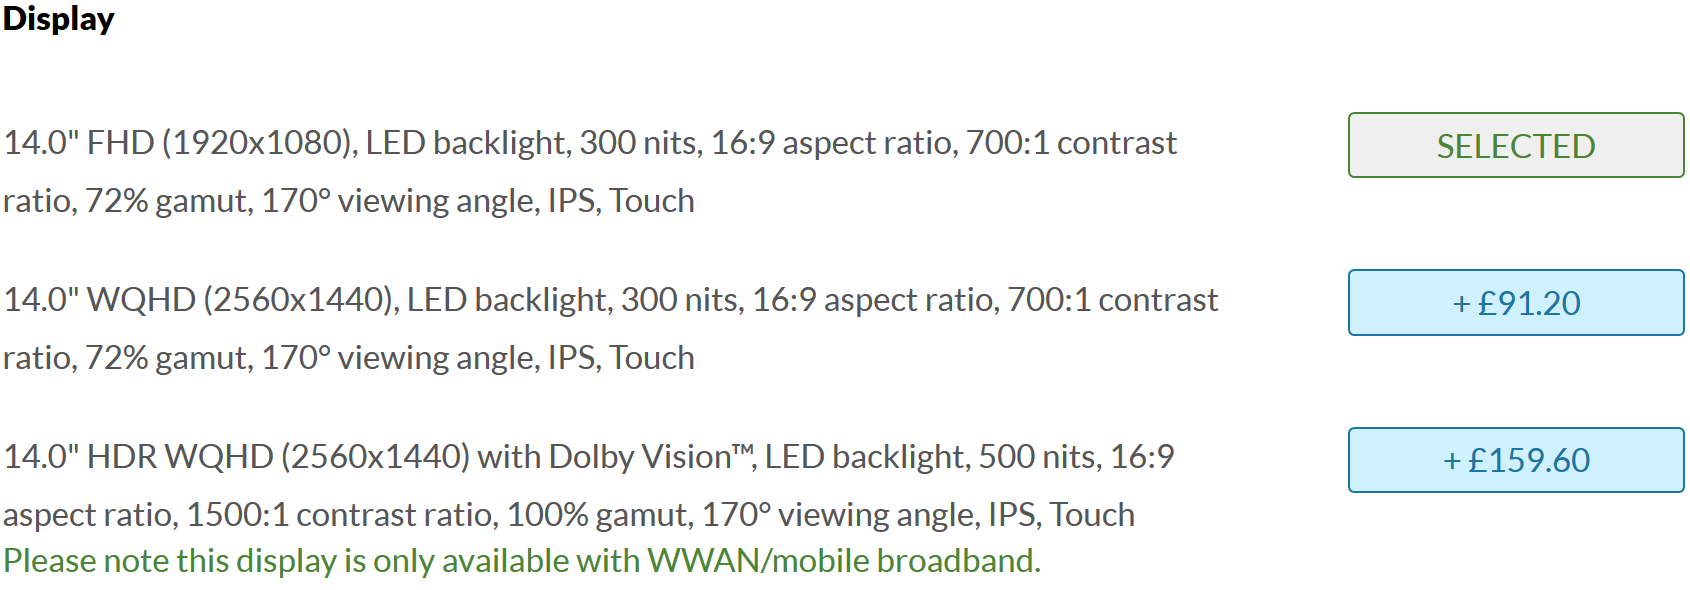
\includegraphics[width=\linewidth]{thinkpad-x1-yoga-display}}\only<2|handout:0>{
\includegraphics[width=\linewidth]{thinkpad-x1-yoga-display-invalidconf}}}}
\end{frame}

\begin{frame}{\myframetitle}
	\partofpage{70}{\myexampletight{Still Configuring a Notebook}{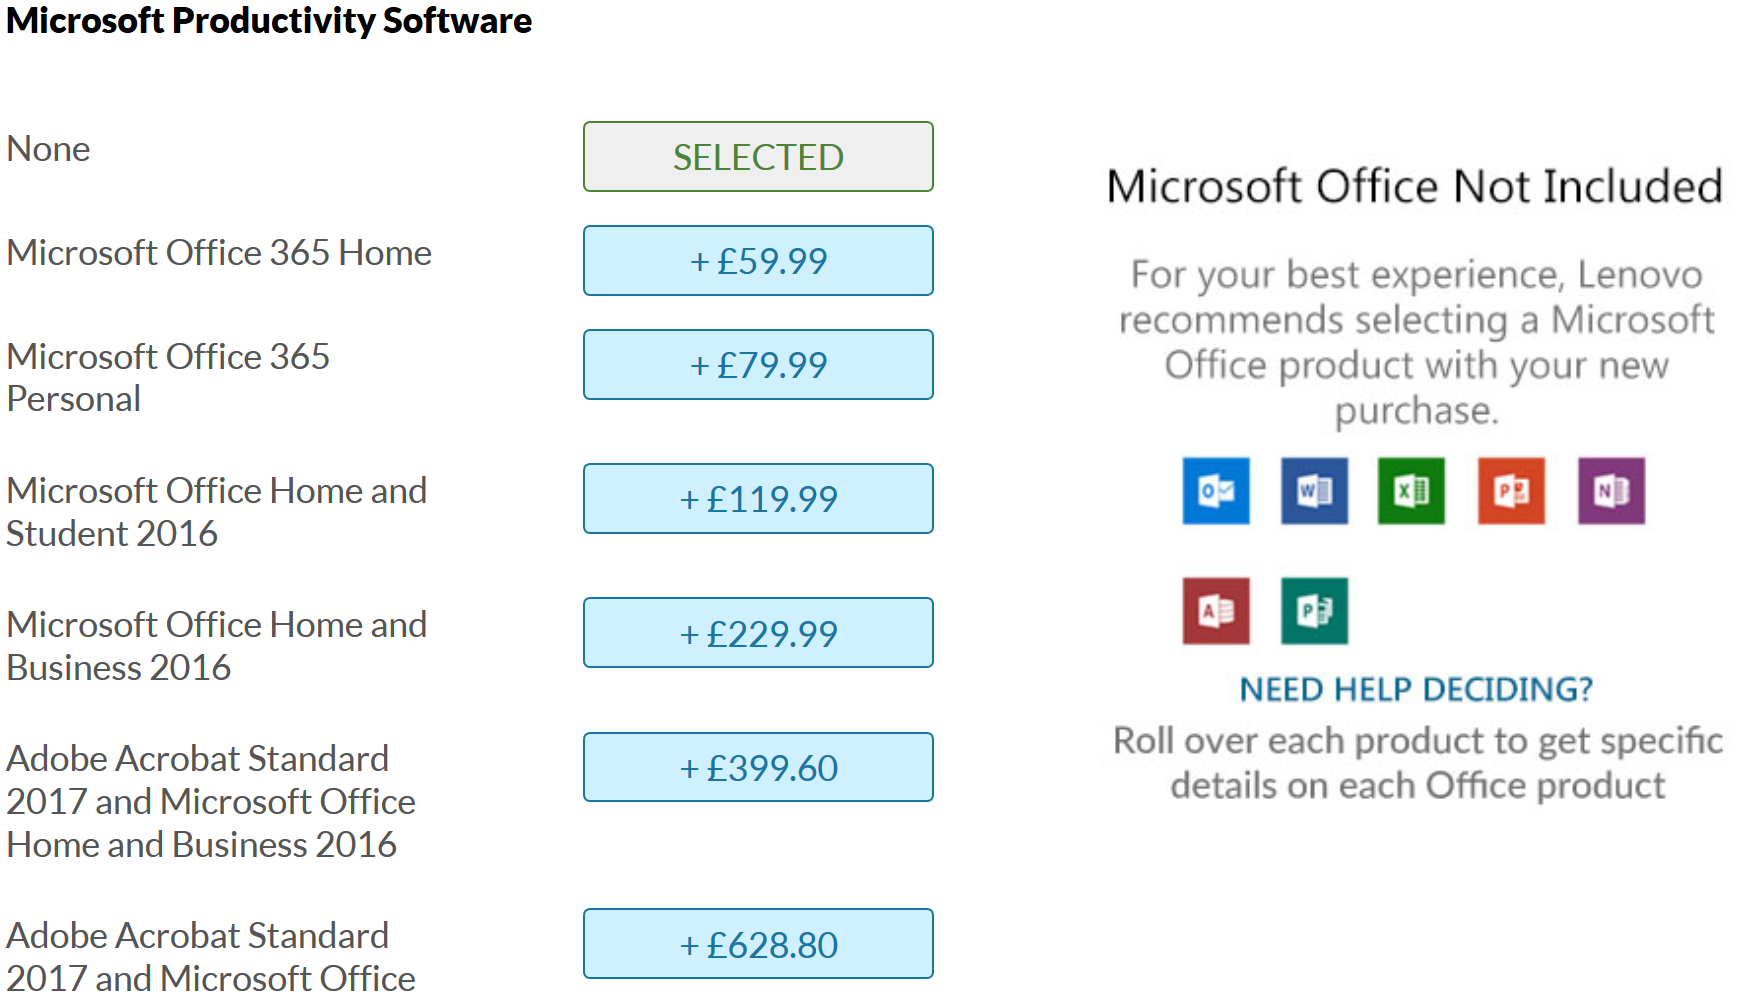
\includegraphics[width=\linewidth]{thinkpad-x1-yoga-office}}}
\end{frame}

\begin{frame}{\myframetitle}
	~\hfill\partofpage{60}{\myexampletight{Configuring a Car}{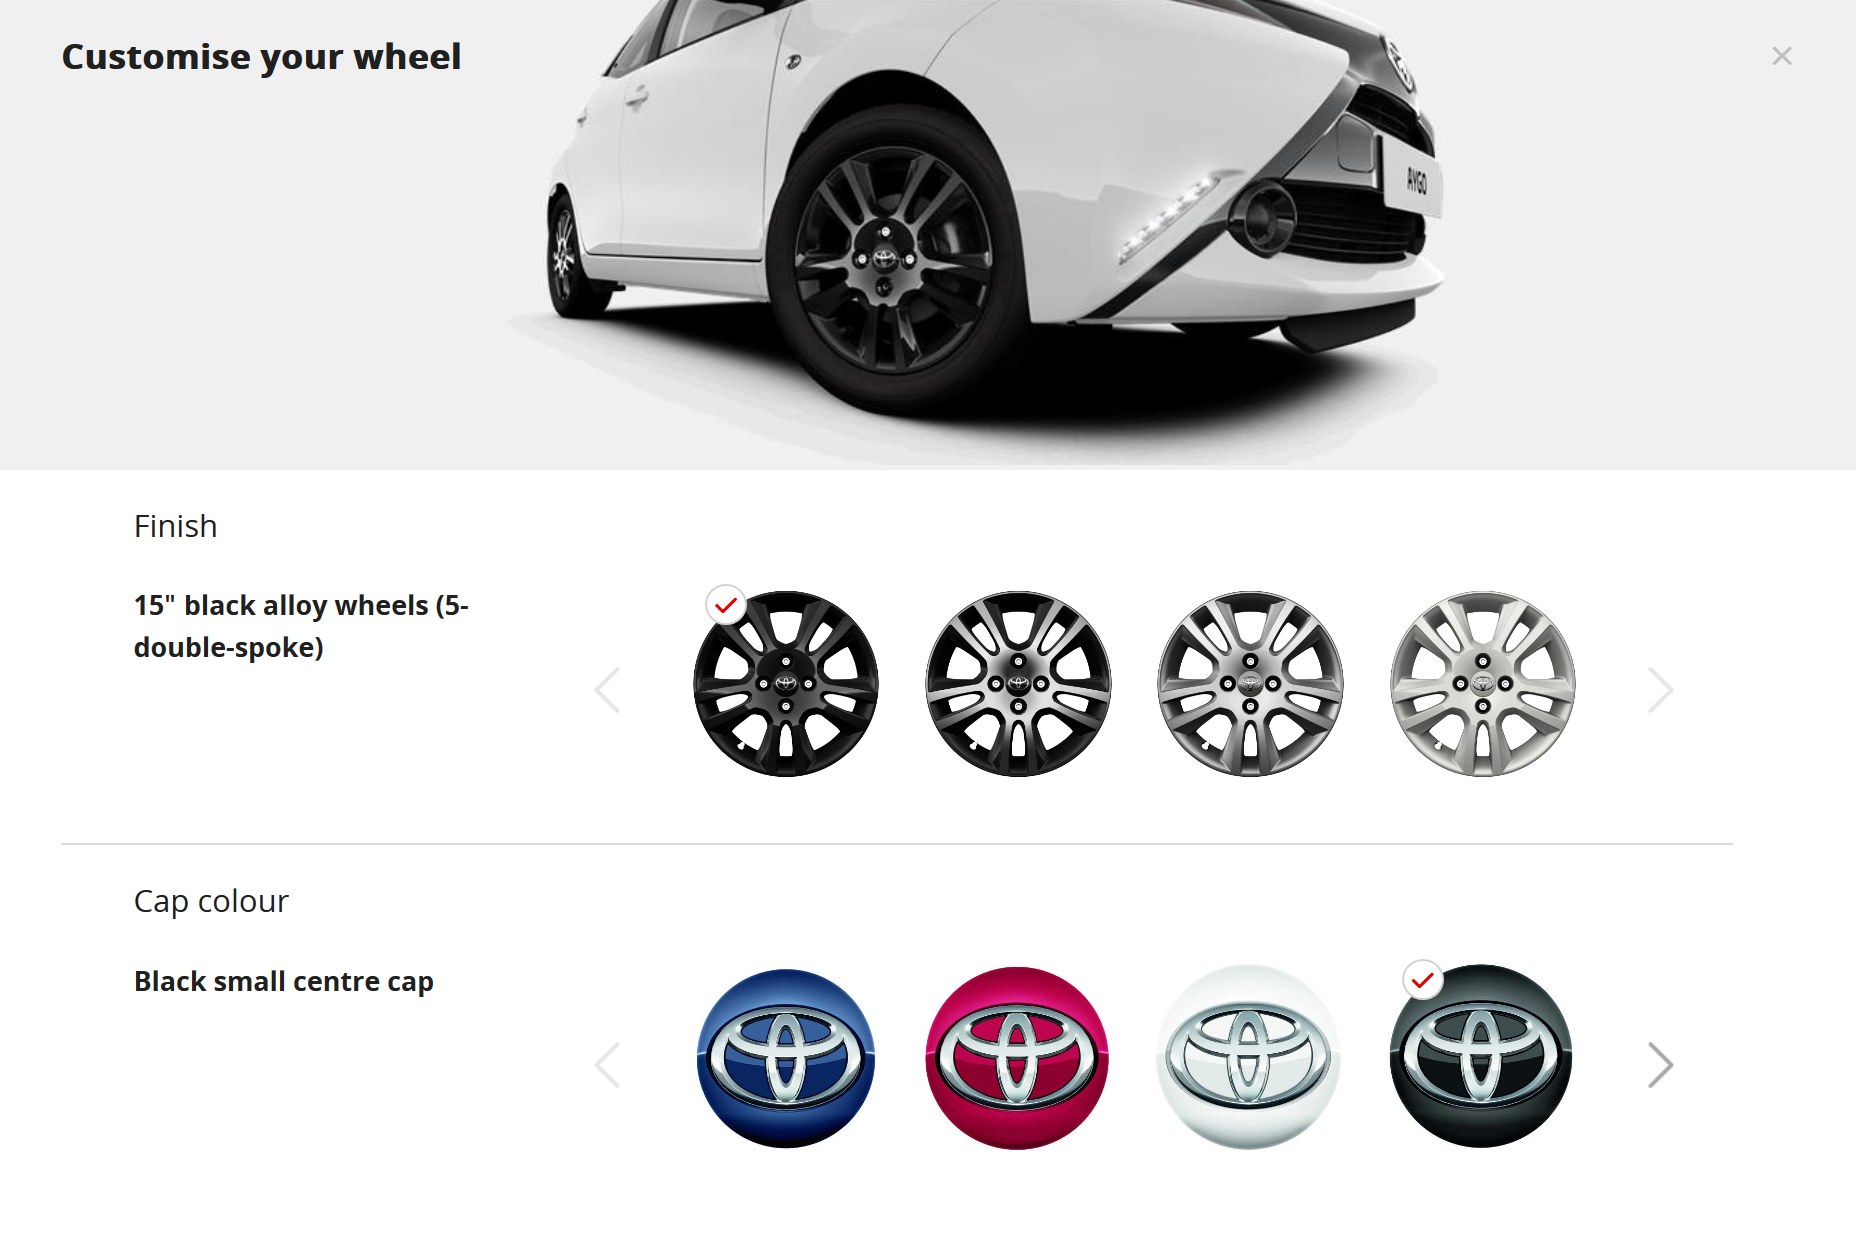
\includegraphics[width=\linewidth]{toyota-aygo-wheels}}}
\end{frame}

\begin{frame}{\myframetitle}
	~\hfill\partofpage{60}{\myexampletight{Configuring a Car with a Weird Price}{\centering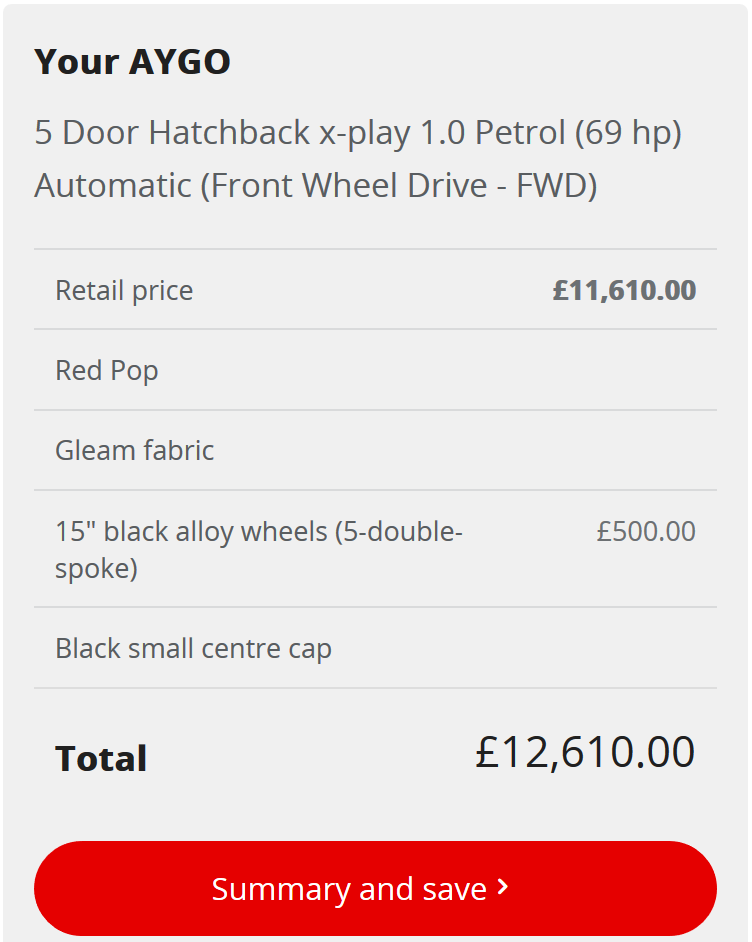
\includegraphics[width=.55\linewidth]{toyota-aygo-costs}}}
\end{frame}

\begin{frame}{\myframetitle}
	~\hfill\partofpage{60}{\myexampletight{Configuring a Car with 8 Wheels!}{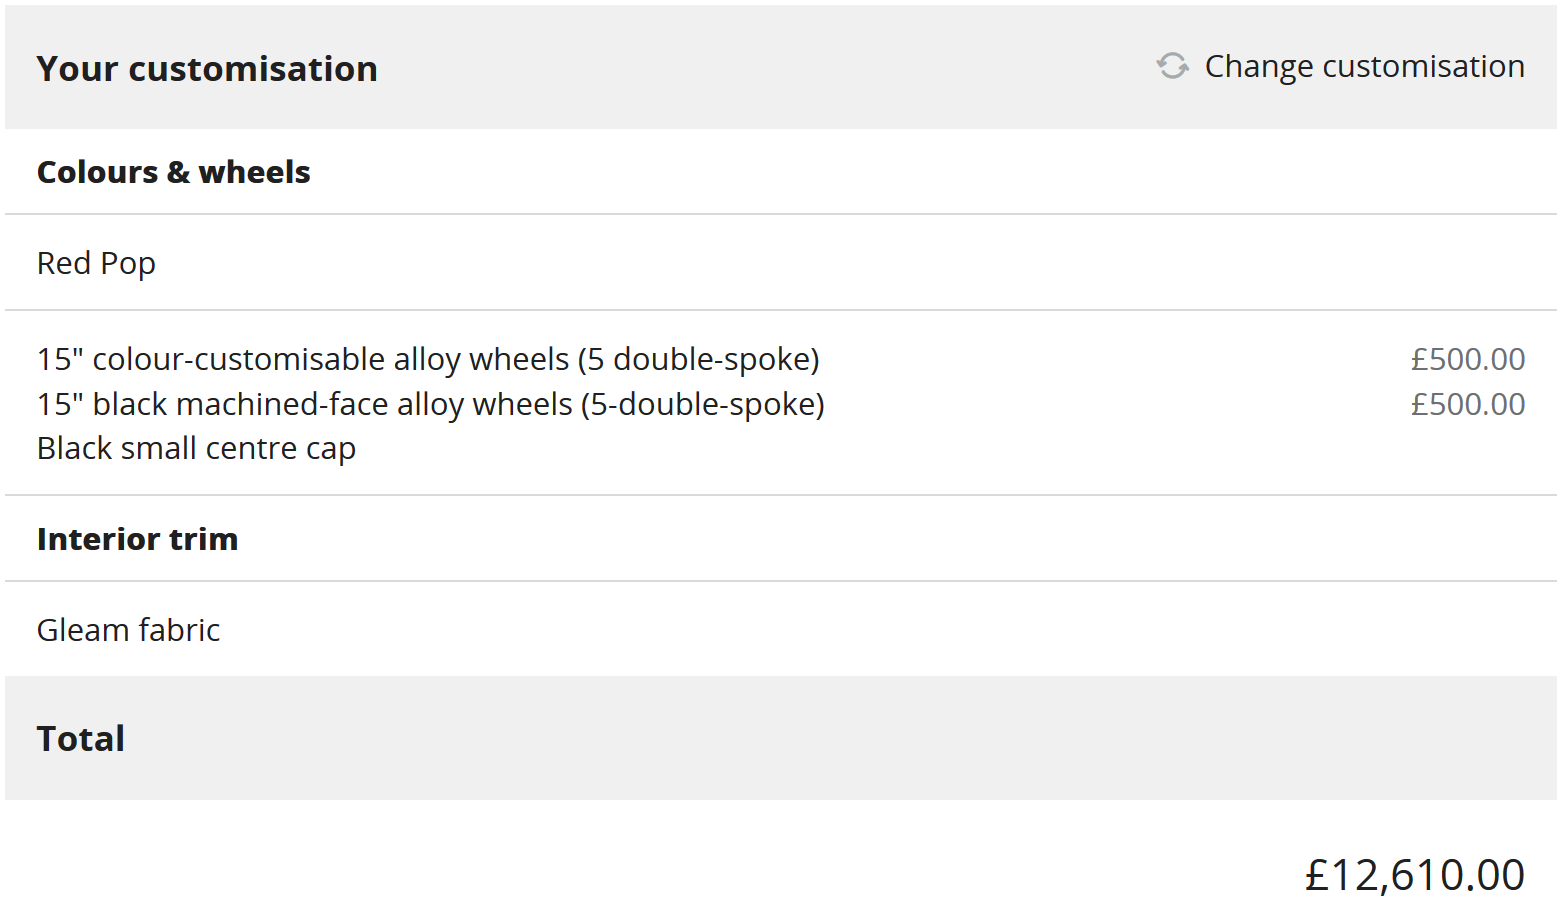
\includegraphics[width=\linewidth]{toyota-aygo-costs3}}}
\end{frame}

\begin{frame}{\myframetitle}
	\partofpage{70}{\myexampletight{Configuring a German Car}{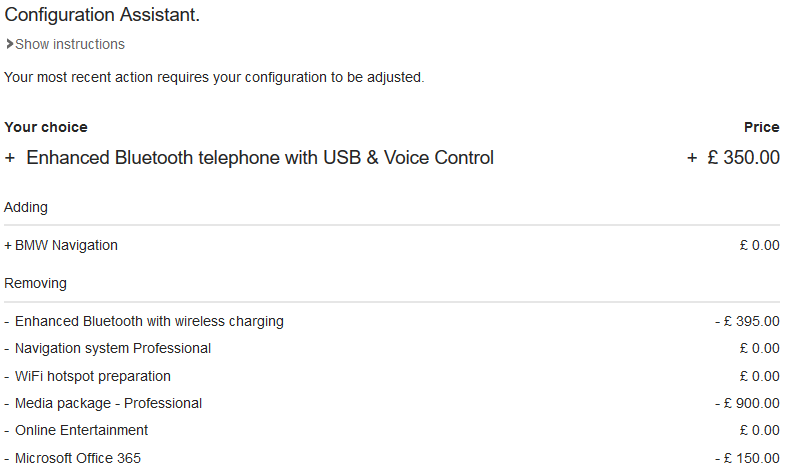
\includegraphics[width=\linewidth]{bmw-series1-confassistant-bluetooth}}}
\end{frame}

% do everything with one running example (preferably the one from before)
% ie, show an example of an inconsistency and then reveal the issue - can be combined with the MUS explanations

% FM [UVL,attribute,cardinalities,...] -> phi[Prop/FOL/QBF...] -> CNF[BDD/d-DNNF/...] -> SAT[#SAT,AllSat] -> SAT Result -> FM Result
% show this + where it can be varied (BDD, ...) at the end

\begin{frame}{\myframetitle}
	this section should teach all usual FM/cfg analyses - some in more detail, some only high-level (other SPL analyses come in analyses.tex)

	list questions we might want to ask a feature model (maybe grouped in the order in which they are discussed)

	include some simple \#SAT questions (e.g., feature prioritization)

	am i developing unused code?

	how to find out whether a partial configuration is valid? (show decision propagation in FeatureIDE)

	etc.
\end{frame}

\subsection{Automated Reasoning with SAT and \#SAT}

\begin{frame}{-- Problem}
	recapitulate (very basic) theory behind both problems

	revisit what the class of programs named "solver" does, and why it is important that we use OTS solvers and profit from their optimizations/contests - idea: reduce practical problems to solvers (sim. to TheoInf/Logics)
\end{frame}

%sat, taut

\begin{frame}{-- Solvers}
	explain simple SAT and \#SAT solver ($SAT(\phi) \in \{\top, \bot\}$)

	as a black-box/abstraction (may be implemented in many ways, e.g. as BDD)

	extensions to SAT solver interface (harder to implement):
	
	when SAT = true, some give a satisfying assignment (for optimizations)
	
	wen SAT = false, some give a MUS (for explanations) % see master theses of T. Günther, S. Ananieva

	\#SAT subsumes SAT, but is harder to compute
\end{frame}

\subsection{Void Feature Model}
\begin{frame}{\myframetitle}
	is the FM even consistent? does it have errors? % can we even get a valid configuration? does a configurator allow anything? a clever configurator would see that

	void iff $SAT(\phi) = \bot$

	for each analysis, also list \#SAT encoding
	to WHICH DEGREE is a FM consistent (i.e., degree of freedom / variability factor)?

	also list explanations / MUS (very shortly)

	maybe for each analysis, list applications/scenarios, here: find grave modeling errors, check wether a configurator even allows to create ANY valid configuration
\end{frame}

\subsection{Core and Dead Features} % + these are variability smells
\begin{frame}{\myframetitle}
	can a feature be chosen at all? is it false-optional?
	to WHICH DEGREE is a feature core/dead? feature prioritization

	f core iff $SAT(\phi and not f) = \bot$
	
	f dead iff $SAT(\phi and f) = \bot$

	applications: find anomalies/inconsistencies (false-optional), commonality, feature prioritization
\end{frame}

\subsection{Partial Configurations}
\begin{frame}{\myframetitle}
	can a partial configuration be completed?
	can also be connected to Chico's \#SAT applications

	note that this is a generalization of void/core/dead

	total configurations were defined before, now expand this definition to a tuple $(sel, desel)$ and explain why

	applications: ...
\end{frame}

\subsection{Redundant Constraints (?)}
\begin{frame}{\myframetitle}
	... % include this? it has no real #SAT equivalent
\end{frame}

\subsection{Other Analyses}
\begin{frame}{\myframetitle}
	list some more analyses/questions

	atomic sets, determinate features

	probably too much:
	FM edits?
	redundant constraints?

	%explanations?
\end{frame}

% maybe combine Challenges/Experiences? or flip them?
\subsection{Challenges}
\begin{frame}{\myframetitle}
	how is SAT (before: a black box) implemented (very broadly)?

	solvers have parameters, heuristics (variable ordering/assignment, restarts, ...)

	there are SAT solvers that do not use CNF, there are other techniques entirely (BDD, d-DNNF)

	CNF/DIMACS transformation

	non-Boolean requires richer theories (SMT, CSP)
\end{frame}

\subsection{Experiences} % performance / efficiency
\begin{frame}{\myframetitle}
	show a few diagrams with performance on large models

	(may even be implemented concretely as BDD)

	only with Boolean formulas can we get really performant results today

	BDDs are hard to build, but have large payoff (maybe one slide on the abstract concept of knowledge compilation, without too many details?)

	most of this is implemented in FeatureIDE, the configurator is a clever combination of the techniques explained above (Boolean constraint/decision propagation) % show linux configurator

		%at the end (what else is there?): in practice, we also have non-Boolean features/attributes/constraints over attributes (more details on efficiency in third block)

	%there is evidence (Knueppel) that the full expressive power of Boolean formulas is needed for real-world formulas

\end{frame}

% end goal: the lecture shows how to realize a automated configurator that does not allow invalid configurations

\subsection{Challenges of Feature Modeling}

\begin{frame}{\myframetitle}
	scoping: which features do we want to deliver? (vl 8,12)

	interactions: which dependencies between feature are there? (vl 9)

	new tools, languages, experts/consultants, ...
\end{frame}

% later on allsat: DNF as opposition? subtractive/additive definition?

% describe sat, #sat, allsat
% describe size of product lines (chico)

% \myexampletight{Industrial Configuration Spaces \mysource{\evaluatingsharpsatsolvers}}{
% 	\centering\evaluatingsharpsatsolverslink{\includegraphics[width=\linewidth,page=6,trim=50 210 320 440,clip]{2020/2020-VaMoS-Sundermann}}
% }